\documentclass[letterpaper,10pt]{article}

% Language setting
% Replace `english' with e.g. `spanish' to change the document language
\usepackage[utf8]{inputenc}
\usepackage[T1]{fontenc}
\usepackage[english]{babel}

% Set page size and margins
% Replace `letterpaper' with `a4paper' for UK/EU standard size
\usepackage[letterpaper,top=2cm,bottom=2cm,left=3cm,right=3cm,marginparwidth=1.75cm]{geometry}

% Useful packages
\usepackage{amsmath}
\usepackage{amssymb}

%\usepackage{stmaryrd}
\usepackage{graphicx}
\graphicspath{ {./} }

\usepackage{biblatex} %Imports biblatex package
%\usepackage[colorlinks=true, allcolors=blue]{hyperref}

\addbibresource{bibliography.bib} %Import the bibliography file


\title{Modular Forms, Elliptic curves and Modular curves}
\author{Armand Perrin, Samy, Damian}

\begin{document}

\maketitle%---------------------------------------------------------------
\part{The Modularity Theorem}

\paragraph{}The modularity theorem was first partially proven by Andrew Wiles in 1995 (before known as the Taniyama-Shimura conjecture) 
and led to a proof of Fermat's Last theorem (1637). The proof was then completed in 2001, showing a strong connexion between 
two kind of objects : modular forms and elliptic curves. In this part we will introduce some notions in order to understand 
the statement of the modularity theorem : 

\paragraph{Theorem } (Modularity Theorem) All elliptic curves over $\mathbb{Q}$ are modular.



\section{Riemann surfaces}%------------------------------------------------------------------------------------------------------------------------------------

\paragraph{Definition 1.1} A $n$-manifold $\mathcal{M}$ is a Hausdorff topological space locally homeomorphic to $\mathbb{R}^n$.
This means that for every point $p \in \mathcal{M}$ there exists an open neighborhood $U$ of $p$ and an homeomorphism $\varphi : U \to \mathbb{R}^n$ to an open subset
of $\mathbb{R}^n$. $(U,\varphi)$ is called a chart.


\paragraph{Definition 1.2} Given two charts $(U,\varphi)$ and $(V,\psi)$ of an $n$-manifold $\mathcal{M}$ with $U\cap V \neq \emptyset$ the map
$\varphi \circ \psi^{-1} : \psi(U\cap V) \subset \mathbb{R}^n \to \varphi(U\cap V) \subset \mathbb{R}^n$ is called a transition map.

{\itshape \paragraph{} We want to extend theses notions to the complex numbers therfore we can replace $\mathbb{R}^n$ by $\mathbb{C}^n$ in the
 two previous definitions to define a complex $n$-manifold. A real $n$-manifold is said to be $\mathcal{C}^k$ if it's transition maps are all $\mathcal{C}^k$ 
 similarly we will consider the complex 1-manifolds whose transition maps are not only smooth but also holomorphic, wich is a much more stronger constraint.}

\paragraph{Definition 1.3} A Riemann surface is a connected complex 1-manifold whose transitions maps are holomorphic.

\paragraph{Definition 1.4} A map $f : \mathcal{M}_1 \to \mathcal{M}_2$ between two Riemann surfaces is said to be holomorphic if for each charts $(U,\varphi),(V,\psi)$
of $\mathcal{M}_1,\mathcal{M}_2$ respectively, the complex function $\psi \circ f \circ \varphi^{-1}$ is holomorphic over $\varphi(U\cap f^{-1}(V))$.

\paragraph{Definition 1.5} (Unformal) \\ Intuitively the genus of a Riemann surface is the number of its holes as a multiple torus. 

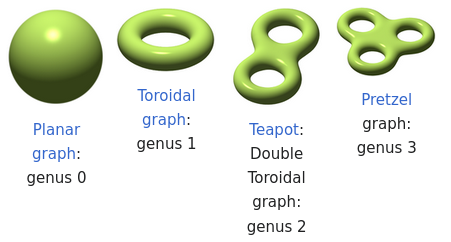
\includegraphics[scale=0.7]{genus}

{\itshape \paragraph{} More formally the genus of $X$ can be defined as half the dimension of $H_1(X,\mathbb{C})$, the first singular homology group.  } 


\paragraph{Theorem 1.6} (Classification of compact Riemann surfaces) \\ 
Two compact Riemann surfaces are homeomorphic to eachother if and only if they have the same genus.


\section{Lattices and complex tori}%------------------------------------------------------------------------------------------------------------------------------------

\paragraph{Definition 2.1} A \textbf{lattice} is a subset of $\mathbb{C}$ of the form $\omega_1\mathbb{Z} \oplus \omega_2\mathbb{Z}$ with $\{\omega_1,\omega_2\}$ a 
$\mathbb{R}$-basis of $\mathbb{C}$. 
{\itshape \paragraph{} This is equivalent to  $\frac{\omega_1}{\omega_2} \notin \mathbb{R}$. We can suppose that $\frac{\omega_1}{\omega_2} \in \mathcal{H}$ for convenience.
}
\paragraph{Definition 2.2} We say that two lattices $\Lambda$ and $\Lambda'$ are isomorphic if there exists an $m\in \mathbb{C}$ such that 
$m\Lambda = \Lambda'$.

\paragraph{Proposition 2.3} Every lattice $\Lambda = \omega_1\mathbb{Z} \oplus \omega_2\mathbb{Z}$ is isomorphic to  $\mathbb{Z} \oplus \tau\mathbb{Z}$ 
for some $\tau \in \mathcal{H}$.\\

{\itshape Proof :} $\omega_1 \neq 0$ so we can consider the isomorphic lattice $(\frac{1}{\omega_1})\Lambda = \mathbb{Z} \oplus \tau\mathbb{Z}$ with 
$\tau = \frac{\omega_2}{\omega_1}$, if $\tau \notin \mathcal{H}$ then $-\tau \in \mathcal{H}$ and $\mathbb{Z} \oplus -\tau\mathbb{Z} = \mathbb{Z} \oplus \tau\mathbb{Z}$.

\paragraph{Proposition 2.4} Two lattices $\Lambda = \mathbb{Z} \oplus \tau\mathbb{Z}$ and $\Lambda' = \mathbb{Z} \oplus \tau'\mathbb{Z}$ are isomorphic if and only if
$\tau' = \gamma \cdot \tau$ for some $\gamma \in SL_2(\mathbb{Z})$.




\paragraph{Definition 2.5} The complex tori associated to a lattice $\Lambda$ is the abelian quotient group $\mathbb{C} / \Lambda$.  

\paragraph{Proposition 2.6} The quotient topology over $\mathbb{C} / \Lambda$ makes it a Riemann surface.

\paragraph{Definition 2.7} An \textbf{isomorphism} of complex tori $\varphi : \mathbb{C} / \Lambda \to \mathbb{C} / \Lambda'$ is a holomorphic 
group isomorphism. $\mathbb{C} / \Lambda$ and $\mathbb{C} / \Lambda'$ are then said to be isomorphic.

\paragraph{Theorem 2.8}  Two complex tori $\mathbb{C} / \Lambda$ and $\mathbb{C} / \Lambda'$ are isomorphic if and only if  $\Lambda$ and $\Lambda'$ are isomorphic.


{\itshape \paragraph{}Remark: The map  $\Psi: \Lambda \mapsto \mathbb{C}/\Lambda$ is  a bijection from the set of lattices to the set of complex tori that
 preserves isomorphism. Therefore, the categories of lattices up to isomorphism and complex tori up to isomorphism are equivalent.
}
\section{Complex tori and elliptic curves}%------------------------------------------------------------------------------------------------------------------------------------
\paragraph{Definition 3.1} Given a sub-field $\mathbb{K}$ of $\mathbb{C}$, an \textbf{elliptic curve} over $\mathbb{K}$ is the set of points $(x,y) \in \mathbb{K}^2$ such that 
\[\ y^2 = 4x^3 - ax - b \] for some $(a,b) \in \mathbb{K}^2$ such that $a^3-27b^2 \neq 0$.
{\itshape \paragraph{} Remark: The condition $a^3-27b^2 \neq 0$ correspond to the curve being smooth.
}

\paragraph{Definition 3.2} An isogeny of elliptic curves is a map  between two elliptic curves such that $ \phi(x,y) = (R_1(x,y),R_2(x,y))$ 
with $R_1$ and $R_2$ two rational fuctions and that is also a group morphism. And an isogeny that is also a group isomorphism is called an isomorphism of
elliptic curves.

\paragraph{Proposition 3.3} If there is an isogeny $\phi$ from $E_1$ to $E_2$ then there is an isogeny
$\psi : E_1 \to E_2$ called the dual isogeny, and we say that $E_1$ and $E_2$ are isogenuous.
This defines an equivalence relation.

{\itshape \paragraph{}Remark: It can be shown that every curve that is the zero set of a polynomial of the form : 
\[ y^2z - (ax^3+bx^2z+ cxz^2 + dz^3)\]
is isogenuous (if we adapt the previous definition) to a curve of the form \[ y^2z - (x^3+bxz^2 + cz^3)\]
whose solutions of the form (x,y,1) satisfies the equation : \[\ y^2 = x^3 + bx + c \]

}



\paragraph{Definition 3.4} Given a complex lattice $\Lambda$, the Weierstrass function $\wp$ is defined by : 
\[\ \wp(z) = \frac{1}{z^2} +  \sum_{\omega \in \Lambda , \omega \neq 0 }\frac{1}{(z - \omega)^2} - \frac{1}{\omega^2} \]
\paragraph{Proposition 3.5} $\wp$ and $\wp'$ are $\Lambda$-periodic.

\paragraph{Theorem 3.6} The Weierstrass function satisfies the differential equation : 

\[\ \wp'^2 = 4\wp^3 - g_2(\Lambda)\wp - g_3(\Lambda) \] for two complex numbers $g_2(\Lambda)$ and $g_3(\Lambda)$.

{\itshape \paragraph{} Proof :} For $z$ close to 0 we have : \begin{align*}
    \wp(z) &= \frac{1}{z^2} +  \sum_{\omega \in \Lambda , \omega \neq 0 }\frac{1}{\omega^2}  \Bigl(\frac{1}{(1 - \frac{z}{\omega})^2} - 1\Bigr) \\
     &=  \frac{1}{z^2} +  \sum_{\omega \in \Lambda , \omega \neq 0 }\frac{1}{\omega^2}  \sum_{n = 1}^\infty (n+1)\frac{z^n}{\omega^n}\\
     &\text{We can change summation order as the series converges absolutely}\\
     &=  \frac{1}{z^2} +  \sum_{n = 1}^\infty (n+1)z^n  \sum_{\omega \in \Lambda , \omega \neq 0 } \frac{1}{\omega^2}\frac{1}{\omega^n} \\
     &=  \frac{1}{z^2} +  \sum_{n = 1}^\infty (n+1)z^n G_{n+2}  \\
     &=  \frac{1}{z^2} +  \sum_{n = 1}^\infty (2n+1) G_{2n+2} z^{2n} \;\; \text{  since  } \forall n \geq 1 \; G_{2n+1} = 0  \\
\end{align*}
Theredore we can compute : \begin{align*}
  \wp'(z) &= -\frac{2}{z^3} + \sum_{n = 1}^\infty (2n+1)2n G_{2n+2} z^{2n-1} \\
  \wp'(z)^2 &= \frac{4}{z^6} - \frac{4}{z^3}\sum_{n = 1}^\infty (2n+1)2n G_{2n+2} z^{2n-1} + \Bigl(\sum_{n = 1}^\infty (2n+1)2n G_{2n+2} z^{2n-1}\Bigr)^2\\
  &= \frac{4}{z^6} - \frac{24G_4}{z^2} + h(z) \;\;\;\; \text{ with h holomorphic on a neighborhood of 0}
\end{align*} On the other hand :
\begin{align*}
  \wp(z) &= \frac{1}{z^2} + 3G_4z^2 + O(z^4) \\
  \wp(z)^3 &= \frac{1}{z^6} + \frac{9G_4z^2}{z^4} + O(1) \\
   4\wp(z)^3 &= \frac{4}{z^6} + \frac{36G_4}{z^2} + g(z)  \;\;\;\; \text{ with g holomorphic on a neighborhood of 0}\\
\end{align*} Then we obtain that $\wp' - 4\wp^3 + 60G_4\wp$ is holomorphic on a neighborhood of 0. But by $\Lambda$-periodicity this function is holomorphic on 
 $\mathbb{C}$. By continuity and $\Lambda$-periodicity it is also bounded on $\mathbb{C}$ and therefore constant.
 Let's denote -$g_3$ this constant (one can show with similar calculations that $g_3 = 140G_6$). We have then :
  \[ \wp'^2 = 4\wp^3 - g_2(\Lambda)\wp - g_3(\Lambda)  \]

\paragraph{Theorem 3.7} The map : \[\ z + \Lambda \to (\wp(z),\wp'(z)) \]
is a bijection from nonzero points of $\mathbb{C} / \Lambda$ to the elliptic curve associated to the equation \[\ y^2 = 4x^3 - g_2(\Lambda)x - g_3(\Lambda) \]

\paragraph{Definition-Proposition 3.8 (Group law)} Given an elliptic curve $E$, $\mathbb{C}/\Lambda$ its associated complex tori and two points $U,V \in E$. There exists
two points $u,v\in\mathbb{C}/\Lambda $ such that $U=(\wp(u),\wp'(u))$ and $ V = (\wp(v),\wp'(v))$. Let's consider the line of $\mathbb{C}^2$ going 
through $U$ and $V$ if $U \neq V$ and the tangent line to $E$ at $U$ if $U=V$. This gives us an line equation of the form \[ ax+ by + c = 0  \]
Lets consider the function $f$ over $\mathbb{C}/\Lambda$ such that: \[ f(z) = a\wp(z) + b\wp'(z) + c \]

We observe that $f$ has zeros at points $u,v$.
If $ b \neq 0$ then $f$ has exactly one other zero $w$ and it is such that  $u + v + w + \Lambda = 0 + \Lambda$.
If $b = 0$ then $u + v + \Lambda = 0 + \Lambda$ then let $w = 0$ and again $u + v + w + \Lambda = 0 + \Lambda$.
Lets define a point $O$ "at infinity" to make notations coherent we denote $(\wp(0),\wp'(0)) := O$.
Thus we define the group law on $E\cup\{O\}$ by : \[ U + V := (\wp(-u - v),\wp'(-u -v)) \]
This makes the map :$  \left\{ \begin{array}{rcl} \mathbb{C}/\Lambda & \longrightarrow & E\cup \{O\} \\
  z + \Lambda & \longmapsto & (\wp(z),\wp'(z)) \\ \end{array} \right. $ a group isomorphism.



\paragraph{Theorem 3.9} Let $E$ and $E'$ be some elliptic curves associated to the lattices $\Lambda$ and $\Lambda'$ respectively,
then the following statements are equivalent :\\

  $i)$ $E$ and $E'$ are isomorphic
  
  $ii)$  $\mathbb{C}/\Lambda$ and $\mathbb{C}/\Lambda'$ are isomorphic.
  
  $iii)$  $\Lambda$ and $\Lambda'$ are isomorphic. \\ 
  
{\itshape \paragraph{}This theorem reduces the problem of parametrization of elliptic curves up to isomorphism to the much simpler problem of parametrization of
 lattices up to isomorphism. In what follows we will identify those 3 categories as the same mathematical objects.
}

\section{Modular curves}%------------------------------------------------------------------------------------------------------------------------------------

{\itshape \paragraph{} In this section we are looking for a moduli spaces (i.e a space that parametrize) of elliptic curves up to isogeny. 
}



\paragraph{Definition 4.1} Let $\Gamma$ be a congruence subgroup of $SL_2(\mathbb{Z})$, we define the modular curve associated to $\Gamma$ by
 $Y(\Gamma) := \{ \Gamma\tau , \tau \in \mathcal{H} \}$ , i.e the set of orbits of the action of $\Gamma$ on $\mathcal{H}$. We also denote $Y_0(N)$ for $Y(\Gamma_0(N))$
 and $Y_1(N)$ for $Y(\Gamma_1(N))$.


\paragraph{Proposition } Each point of $Y(SL_2(\mathbb{Z}))$ correspond to a unique elliptic curve isomorphism class.

{\itshape \paragraph{}Proof : } Points $\tau, \tau' \in \mathbb{C}$ are in the same orbit iff $\tau' = \gamma \cdot \tau$ for some $\gamma \in SL_2(\mathbb{Z})$.
This is equivalent by proposition  2.4 to $\mathbb{Z} \oplus \tau\mathbb{Z}$ and $\mathbb{Z} \oplus \tau'\mathbb{Z}$ being isomorphic.



{\itshape \paragraph{} This last proposition says that $Y(SL_2(\mathbb{Z}))$ is a moduli space of elliptic curves up to isomorphism, we will now answer the question :
what classes of elliptic curves does the modular curves $Y_0(N)$ and $Y_1(N)$ represent ?  } 

\paragraph{Definition } We call a pair $(E,p)$ a pointed elliptic curve if $E$ is an elliptic curve and $p$ is a $N$-torsion point on $E$ 
(seen as an abelian quotient group $\mathbb{C}/ \Lambda$). And we say that two pointed elliptic curves $(E,p)$ and $(E',p')$ are isomorphic if there is an isomorphism
$\phi: E\to E'$ such that $\phi(p) = p'$.

\paragraph{Definition } We call a pair $(E,C)$ an enhanced elliptic curve if $E$ is an elliptic curve and $C$ is a cyclic subgroup of $E$ of order $N$. 
And we say that two enhanced elliptic curves $(E,C)$ and $(E',C')$ are isomorphic if there is an isomorphism
$\phi: E\to E'$ such that $\phi(C) = C'$.

\paragraph{Theorem }\textbf{(Moduli spaces $Y_1(N)$ and $Y_0(N)$ )} \\- Each point of $Y_1(N)$ correspond to a unique pointed elliptic curve isomorphism class.\\
 - Each point of $Y_0(N)$ correspond to a unique enhanced elliptic curve isomorphism class.

 {\itshape \paragraph{} It follows from Chow's theorem and the Rieman-Roch theorem that compact Riemann surfaces are complex algebraic curves,
  this and Theorem 1.6 gives us motivation to make $Y(\Gamma) $ a compact Rieman surface. }


\paragraph{Definition } The fundamental domain $\mathcal{D} \subset \mathcal{H}$ of the modular form $Y(\Gamma)$ is
a region that contains exactly one point from each orbit of $\Gamma$ action except some
possible duplication on the edge.

\paragraph{Proposition} The region $\mathcal{D} = \{ \tau \in \mathcal{H}\;  |\tau| \geq 1 \; and \; |Re(\tau)| \leq 1/2\}$ is a fundamental domain for $Y(SL_2(\mathbb{Z}))$.

{\itshape \paragraph{} After identification of duplicate points on the edge we see that $Y(SL_2(\mathbb{Z})) \simeq SL_2(\mathbb{Z})\backslash \mathcal{D}$ is a punctured sphere.
}

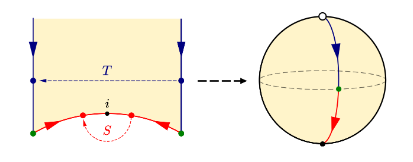
\includegraphics[scale=1.0]{sphere}

\paragraph{Proposition}  $Y(SL_2(\mathbb{Z}))$ can be made a Riemann surface and compactified into $X(1)$ by adding a point at infinity.



\paragraph{Proposition} Similarly for any congruence subgroup $\Gamma$, $Y(\Gamma)$ can be made a Riemann surface and compactified into $X(\Gamma)$
 by adding a finite number of points. We will denote $X(\Gamma_0(N))$ as $X_0(N)$ for any integer $N$. 

\paragraph{Definition} A complex elliptic curve $E$ is said to be \textbf{modular} if there exists an integer $N$ such that there is a surjection holomorphic map $\varphi$ 
from the modular curve $X_0(N)$ to $E$ as Riemann surfaces. $\varphi$ is the called a modular parametrization of $E$.

\paragraph{TODO} congruence subgroup, ex ref \cite{zhou} $G_2$ $g_2(\Lambda)$ Eisenstein series genus...


\printbibliography %Prints bibliography

\end{document} 